\section{Problem Setup and Calibrated Observation Model}

\subsection{Linear Observation Model Under Fixed Shifts and Physical Limits}

Consider an LWIR camera that images a chip under micro-scanning. A motorized stage translates the scene frame-by-frame on a 2D raster grid with sub-pixel steps, producing $K$ low-resolution (LR) temperature frames. Let $x \in \mathbb{R}^{N}$ denote the target high-resolution (HR) temperature image on a $2\times$ output grid. The $k$-th observation is modeled as
\[
y_k = D\,B\,H\,S_{t_k}\,x + n_k,\qquad k = 1,\ldots,K.
\]

The operators are, in order: $S_{t_k}$, shift-and-resample on the HR grid using the refined sub-pixel displacement $t_k$; $H$, optical point spread function (PSF) convolution, modeled as Gaussian with standard deviation $\sigma$ reported in LR pixels and converted when implemented on the HR grid (Appendix~A.5.2); $B$, detector-aperture box integration; and $D$, HR-to-LR downsampling. The noise term $n_k$ models detector read noise, with nominal scale given by the measured $0.0724\,^\circ\mathrm{C}$ noise floor. Thermal drift, alignment residuals, and PSF mismatch are treated as model errors and handled separately via session gating, quality gates, and ablation. In the analysis below, $t_k$ is treated as fixed; in practice it comes from stage priors plus data-driven refinement, not from using stage commands as alignment ground truth. Joint estimation of shifts and image is outside the fixed-linear-operator SVD scope studied here.

Stacking all $K$ frames defines
\[
A=\begin{bmatrix}A_1\\ \vdots\\ A_K\end{bmatrix},\qquad A_k=D\,B\,H\,S_{t_k}.
\]
The structure of $A$---its band-limited attenuation, alias folding, and induced null-space directions---governs both our method design and experimental analysis.

\begin{figure}[t]
  \centering
  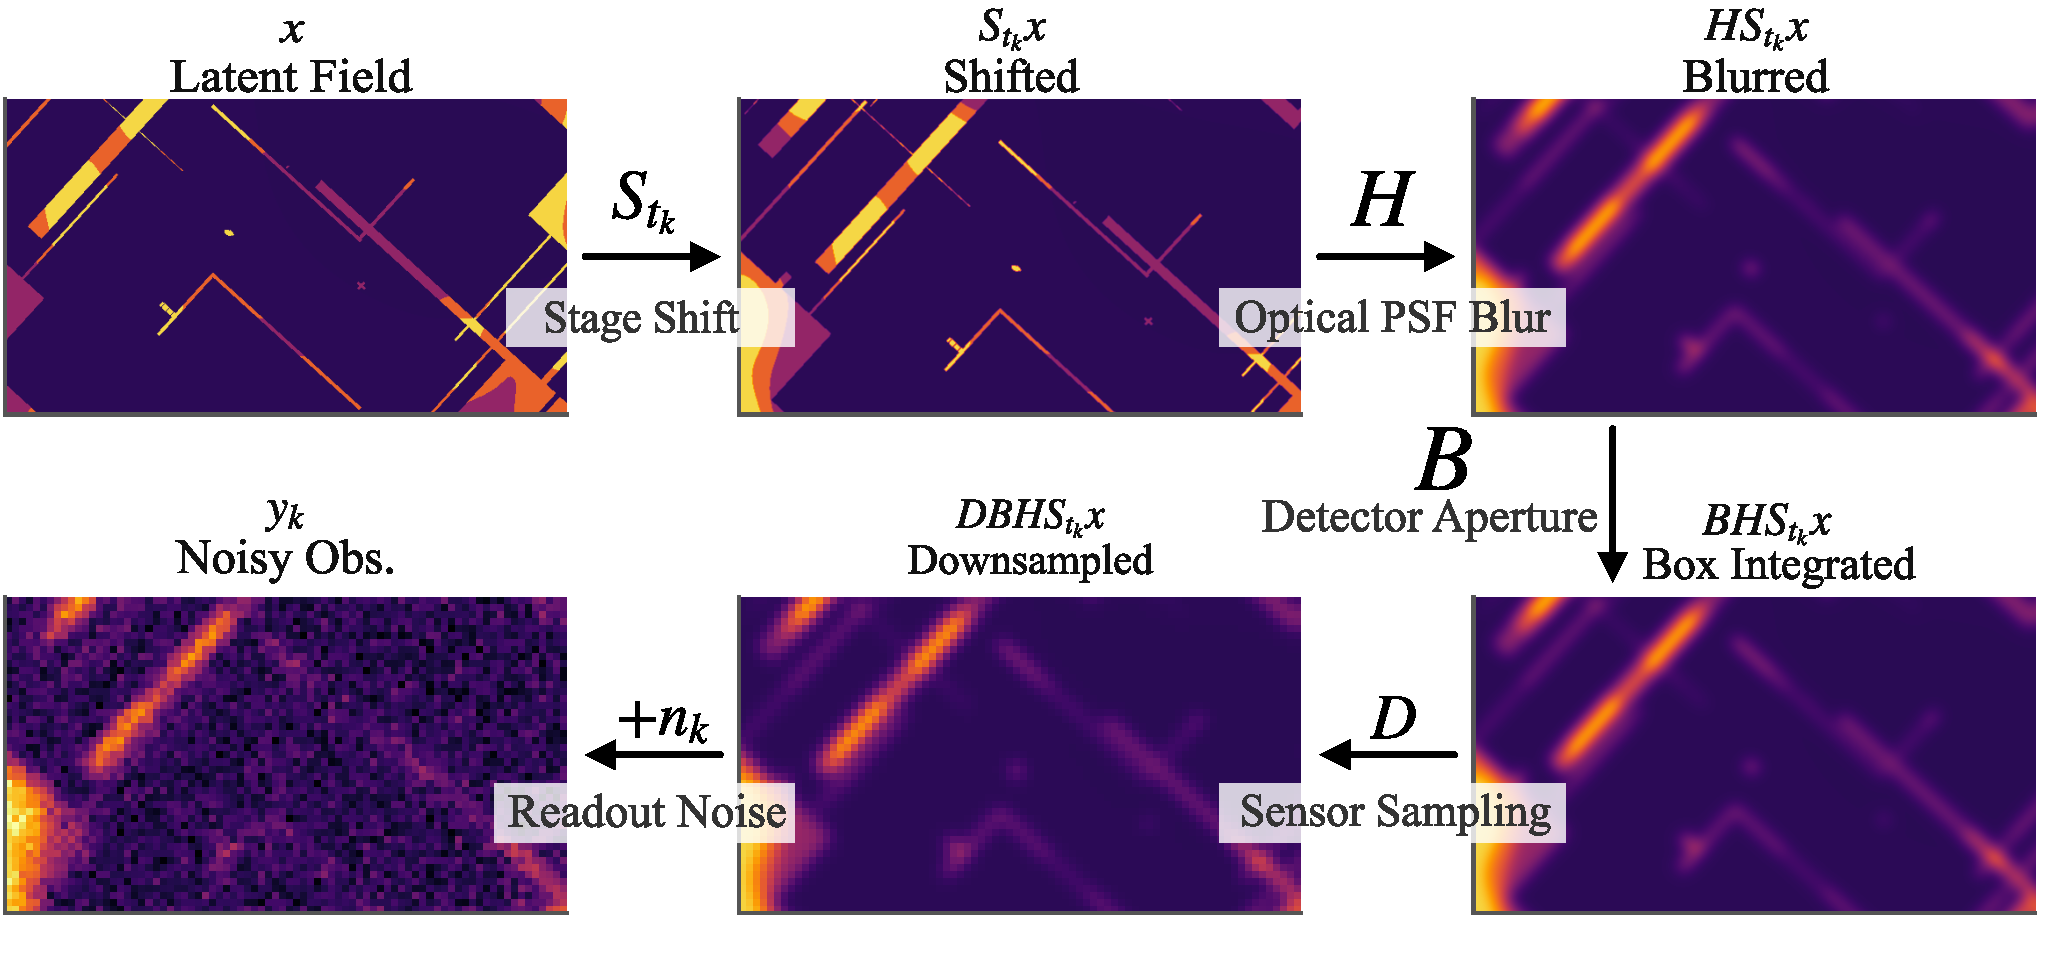
\includegraphics[width=\linewidth]{../figures/observation_pipeline.pdf}
  \caption{Calibrated observation model: single-frame operator chain $S_{t_k}\!\to\!H\!\to\!B\!\to\!D$ and stacked observation operator $A$.}
  \label{fig:obs-pipeline}
\end{figure}

Three scales must be strictly distinguished: detector sampling pitch (sample-plane length per pixel), spatial resolution (minimum resolvable structure set jointly by diffraction, PSF, and detector aperture; about twice the pitch), and output-grid sampling (pixel spacing of the $2\times$ reconstruction grid). These are different physical quantities and are not interchangeable.

This distinction sets feasibility boundaries directly. System transfer is jointly controlled by optical PSF, detector aperture, and sampling. Appendix~A.1 reports Gaussian-PSF envelope, detector-box sinc attenuation, measured thermal contrast, and noise floor separately, to avoid over-interpreting one frequency point as a full-band conclusion. The resulting prediction is that a $2\times$ output grid can support contour-level enhancement only under conditions jointly constrained by FRC and MTF--SNR, while $4\times$ falls into a noise-dominated regime except under optimistic assumptions. This prediction is consistent with the negative $4\times$ network results (Sec.~5.7, Appendix~D.4.2).

MTF--SNR crossing is necessary but not sufficient: it only guarantees that information is not completely annihilated in the forward chain. It does not guarantee reliable recovery under model mismatch, alignment error, and thermal drift.

PSF calibration itself has non-negligible uncertainty. Three independent calibration routes disagree beyond tolerance; arbitration yields only a credible interval (Appendix~A.5.2). Therefore, all PSF-dependent computations---forward modeling, synthetic training data generation, and classical deconvolution---must either scan this interval or explicitly report the chosen $\sigma$.

\subsection{Exact Null Space, \texorpdfstring{$\epsilon$}{epsilon}-Null Space, and Forward-Consistency Blind Spots}

The key implication of the model is not only what can be transmitted, but also which HR perturbations are invisible or nearly invisible to all observations.

The null space $\ker(A)=\bigcap_{k=1}^{K}\ker(A_k)$ contains all HR perturbations that leave all $K$ observations unchanged. These unidentifiable directions come from two mechanisms. First, optical PSF and detector aperture form a pre-sampling transfer function that strongly attenuates high frequencies or fully suppresses frequencies at transfer zeros; directions pushed below noise enter a numerical $\epsilon$-null space (band-limited attenuation). Second, downsampling folds multiple HR frequencies into the same LR band; in single-frame, poorly phase-covered, or weak-transfer alias blocks, this creates cancellation directions or small-singular-value directions (alias folding). Multi-frame phase diversity adds constraints, shrinking the exact null space and improving singular values in well-covered alias blocks, but it cannot recover frequencies jointly annihilated or noise-submerged by the shared pre-sampling transfer function (Appendix~A.2).

Beyond exact null directions, the $\epsilon$-null space
\[
\mathcal{N}_{\epsilon}=\mathrm{span}\{v_i:\sigma_i\le\epsilon\},
\]
where $\sigma_i$ are singular values of $A$, is equally important. Along these near-zero singular directions, sensitivity of observation-domain losses and recovery curvature vanish as $\sigma_i\to 0$ (Appendix~A.2, Propositions P2--P3). Hence:

Any observation-domain loss that compares predictions and measurements only through fixed linear operator $A$ is exactly invariant to components in $\ker(A)$. If the loss is Lipschitz over the residual range of interest, its change along unit components in $\mathcal{N}_{\epsilon}$ is at most $O(\epsilon)$. Applying bounded band weighting in observation space---highpass, full-band, or otherwise---can only scale this bound by a finite factor; for quadratic data terms, recovery curvature along singular directions still vanishes with $\sigma_i^2$, and cannot create non-vanishing restoring force in near-null directions.

This directly limits no-HR-ground-truth evaluation. The most intuitive metric---reprojecting reconstruction into observation space and comparing with measured observations (forward consistency)---is only an observation-space sanity check. It provides zero information on exact-null components and only weak, often noise-dominated information on near-null components. Therefore, low forward residual alone cannot prove clearer SR, nor rank checkpoints without HR truth. Without extra priors or physical constraints, changing HR along exact-null directions does not change any LR observation; amplitudes in these directions are set only by constraints outside the observation model.

On real data, we observe forward loss staying near the noise floor while proxy metrics continue drifting, consistent with drift projecting mainly onto near-null directions. This is a conditional diagnosis, not a theorem about UNet or SGD dynamics. It also defines method boundaries: loss-side forward anchoring alone cannot certify HR details. We therefore use two practical mitigations: injecting multi-frame sub-pixel phase evidence into the input representation (hybrid drizzle input, Sec.~4.4.3), and selecting checkpoints with a mechanized protocol before proxy drift accumulates (Sec.~4.5). Neither removes null-space ambiguity; both reduce near-null drift risk in no-HR-truth settings.

Based on this analysis, our claim boundary is contour-level enhancement on a $2\times$ output grid, making internal chip structures clearer and more stable. We explicitly do not claim:
\begin{enumerate}
\item $5\,\ensuremath{\mu m}$ sampling spacing on a $2\times$ grid does not imply $5\,\ensuremath{\mu m}$ spatial resolution; the latter remains optics-limited.
\item No temperature-metrology claim is made; we evaluate contour visibility and stability, not absolute temperature accuracy.
\item The finest internal structures lie near system resolution limits; full recovery is not physically expected. The question is whether contours are clearer and more stable than LR or bicubic under honest quantitative gates.
\end{enumerate}

Full hardware parameters, acquisition protocol, calibration chain (rotation angle, PSF interval, noise floor), and uncertainty analysis are given in Appendix~B. Alignment pipeline and quality gates are in Appendix~B.2; micro-scan kinematics and thermal-drift analysis are in Appendix~B.3.

\subsection{Overview of Main-Text Evaluation Metrics}

We use three no-reference metric families in the main text. Split-half FRC stratifies the 248 frames by sub-pixel phase into two halves and reconstructs them independently; frequency-domain correlation between halves and periodic-band readings from \texttt{frc\_band\_table.csv} quantify FRC band consistency (definitions and controls in Appendix~A.4). The proxy pair consists of artifact score (lower typically means fewer high-frequency artifacts) and raw-control correlation (higher typically means closer to conservative control). They are drift thermometers and checkpoint-selection signals, not HR truth; the constructive anti-correlation mechanism is detailed in Appendix~A.3. Zigzag-profile metrics measure FWHM and dip depth along a fixed central zigzag cross-section for structure-level contour gating; full profile protocol appears in Appendix~C.6.
